\appendix

\pagenumbering{Roman}

\chapter{Appendix}


\section{Source Code}
\begin{lstlisting}[caption={Implementation of EventBus (Kotlin - HeartrateEventBus)}]
object HeartrateEventBus {
    private val listeners = mutableListOf<(HeartrateEvent) -> Unit>()

    fun subscribe(listener: (HeartrateEvent) -> Unit) {
        listeners.add(listener)
    }

    fun unsubscribe(listener: (HeartrateEvent) -> Unit) {
        listeners.remove(listener)
    }

    fun publish(event: HeartrateEvent) {
        listeners.forEach { listener ->
            listener.invoke(event)
        }
    }
}
\end{lstlisting}

\begin{lstlisting}[caption={Implementation of calorie calculation (Kotlin - ExerciseService)}]
private fun calculateCalories(exercise: Exercise): Float {
    return if (user.gender == Gender.MALE) {
        (exercise.duration * (0.6309*exercise.averageHrBpm!! + 0.1988*user.weight + 0.2017*user.getAge() - 55.0969) / 4.184).toFloat()
    } else {
        (exercise.duration * (0.4472*exercise.averageHrBpm!! + 0.1236*user.weight + 0.074*user.getAge() - 20.422) / 4.184).toFloat()
    }
}
\end{lstlisting}

\section{Supplemental Figures}
\begin{figure}[H]
    \centering
    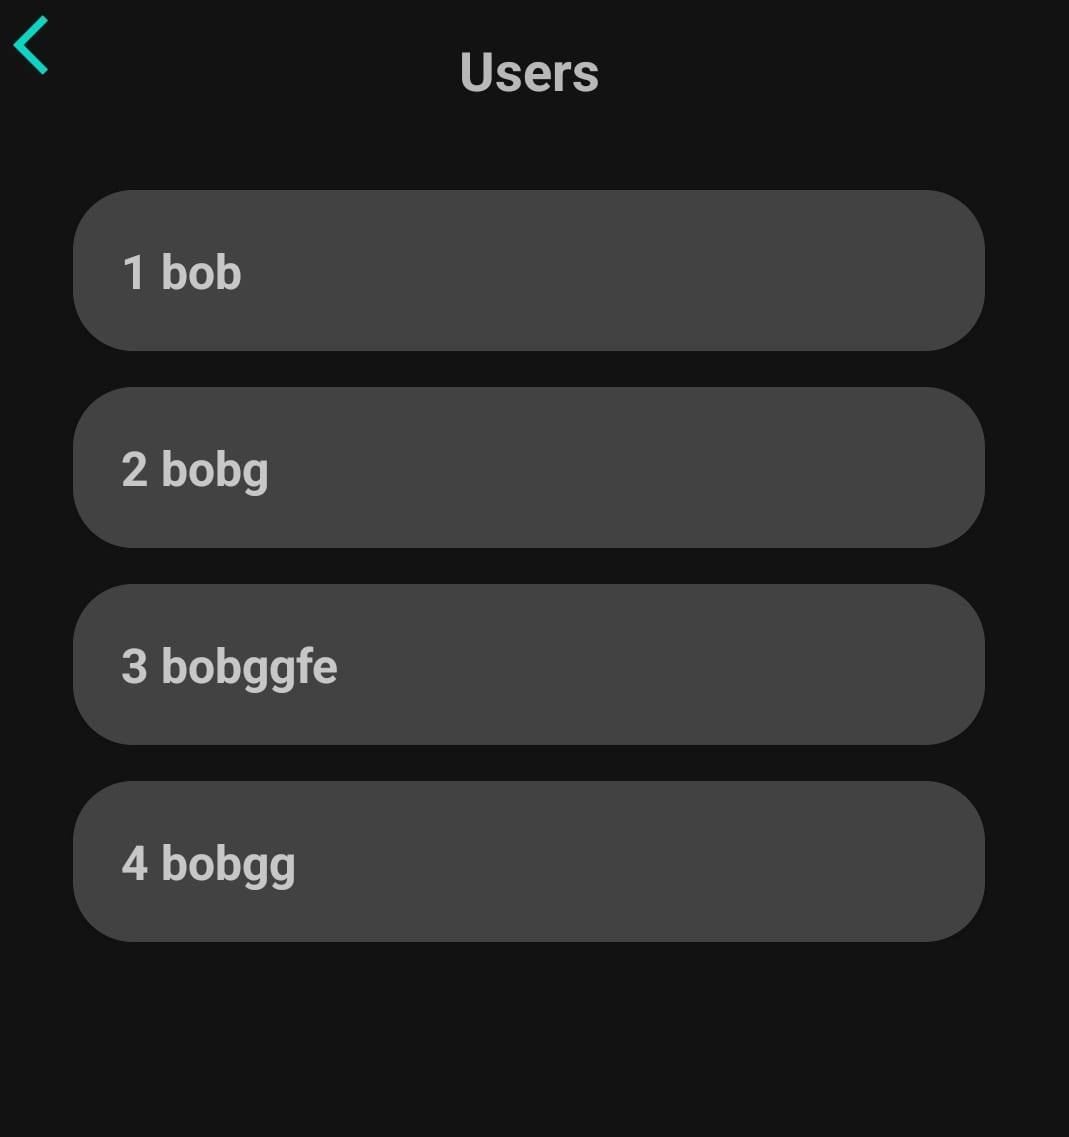
\includegraphics[width=0.7\textwidth]{images/userlistfragment-screenshot.jpeg}
    \caption{Screenshot of UserListFragment containing all users}
    \label{fig:userlistfragment}
\end{figure}